\subsection{Messergebnisse und Auswertung}
Die Counts $N$ sind poissonverteilt, der Fehler beträgt demnach $s_N = \sqrt{N}$. Die Fehler sind in den Graphen der Spektren nicht eingezeichnet, 
da dies zu unübersichtlich ist. Bei den Fits der einzelnen Peaks sind die Fehler eingezeichnet, um die Übereinstimmung der gemessenen Werte 
mit dem theoretischen Modell zu visualisieren.
\subsubsection{CdTe-Detektor}
\paragraph{Spektren}
Die Spektren von \co\ und \am\ sind in \autoref{img:cdte:co:spektrum} und \autoref{img:cdte:am:spektrum} dargestellt. Man erkennt den 59.5\,keV-Peak 
von \am\, bei Kanal 300, den 122.06\,keV-Peak von \co\, bei Kanal 600 und den 136.47\,keV-Peak von \co\, bei Kanal 700.
\begin{figure}[H]
\begin{center}
  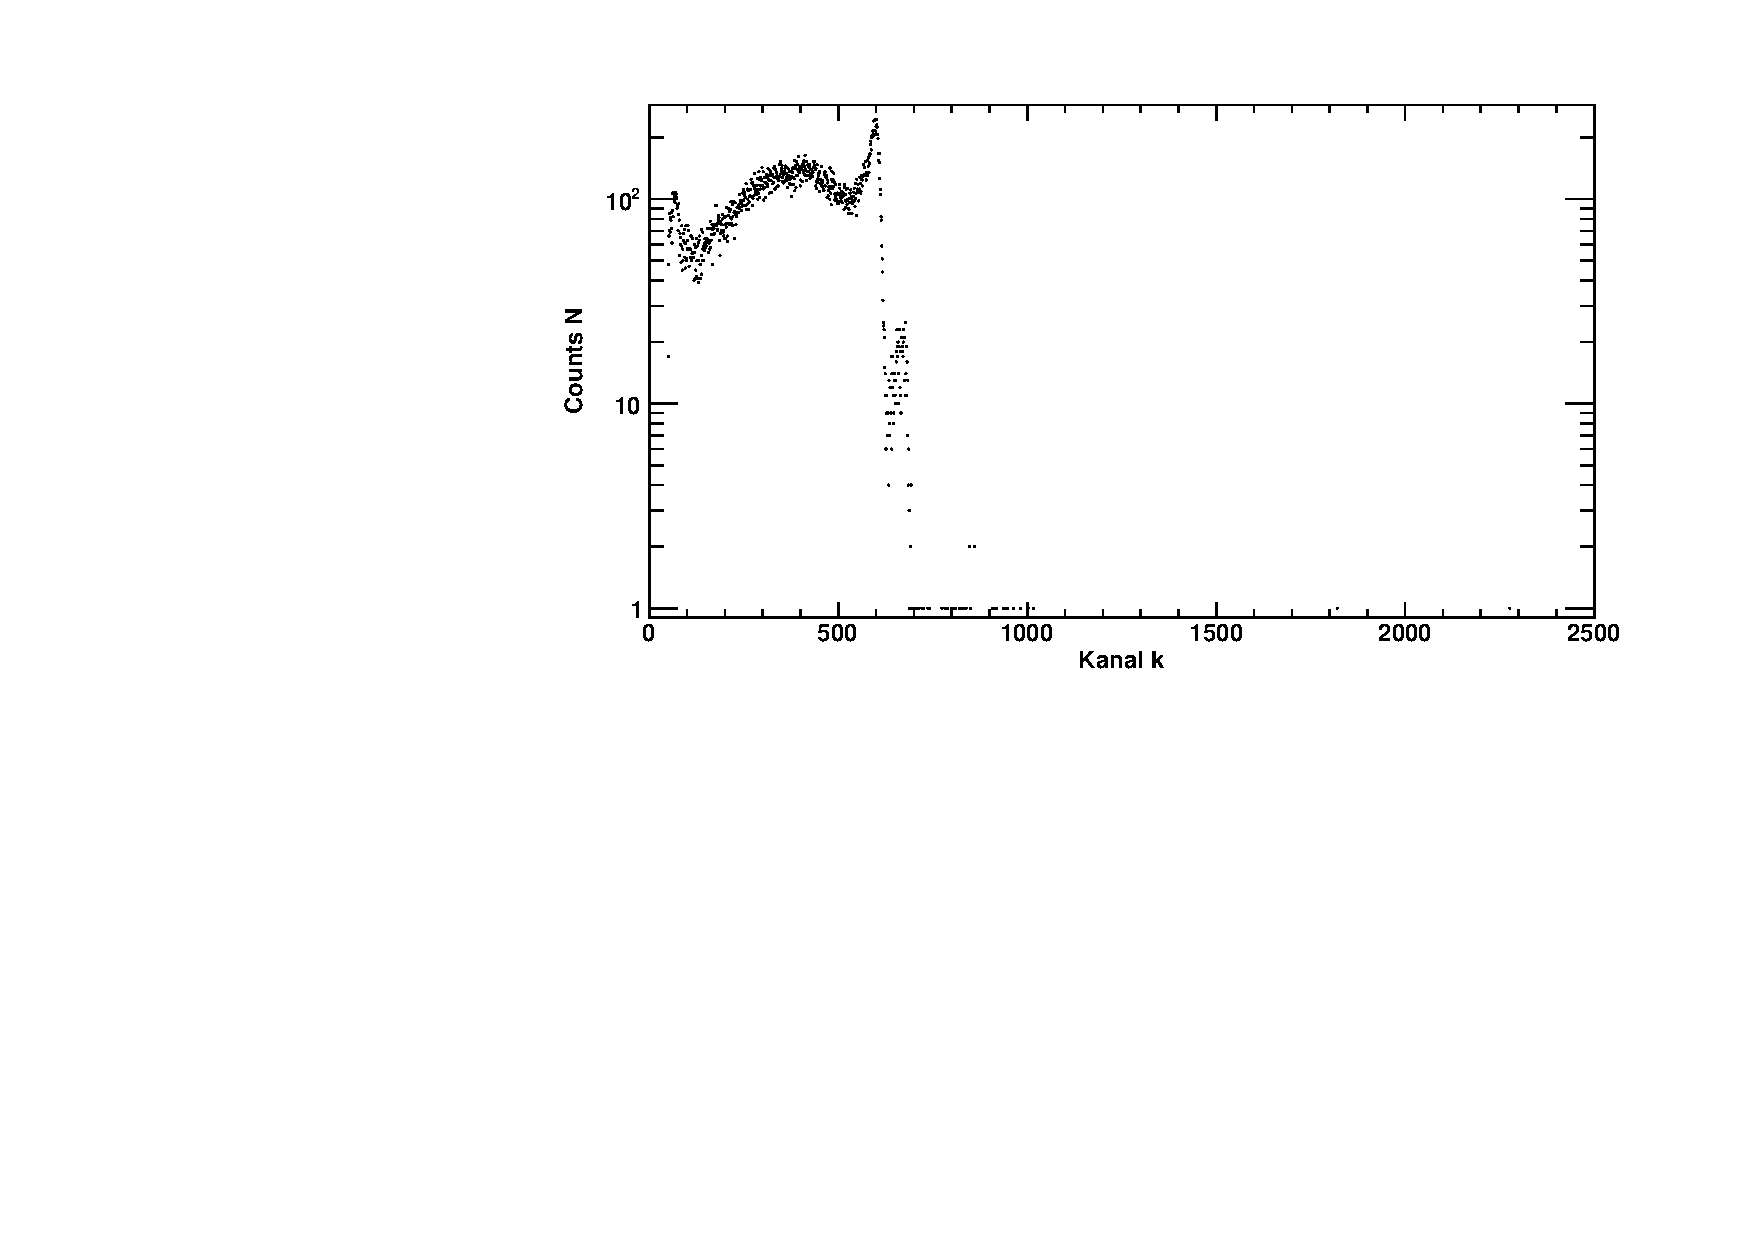
\includegraphics[width=0.95\textwidth]{../img/part3/Co-CdTe_spectrum.pdf}
  \caption{Spektrum von \co, gemessen mit dem CdTe-Detektor.}
  \label{img:cdte:co:spektrum}
\end{center}
\end{figure}

\begin{figure}[H]
\begin{center}
  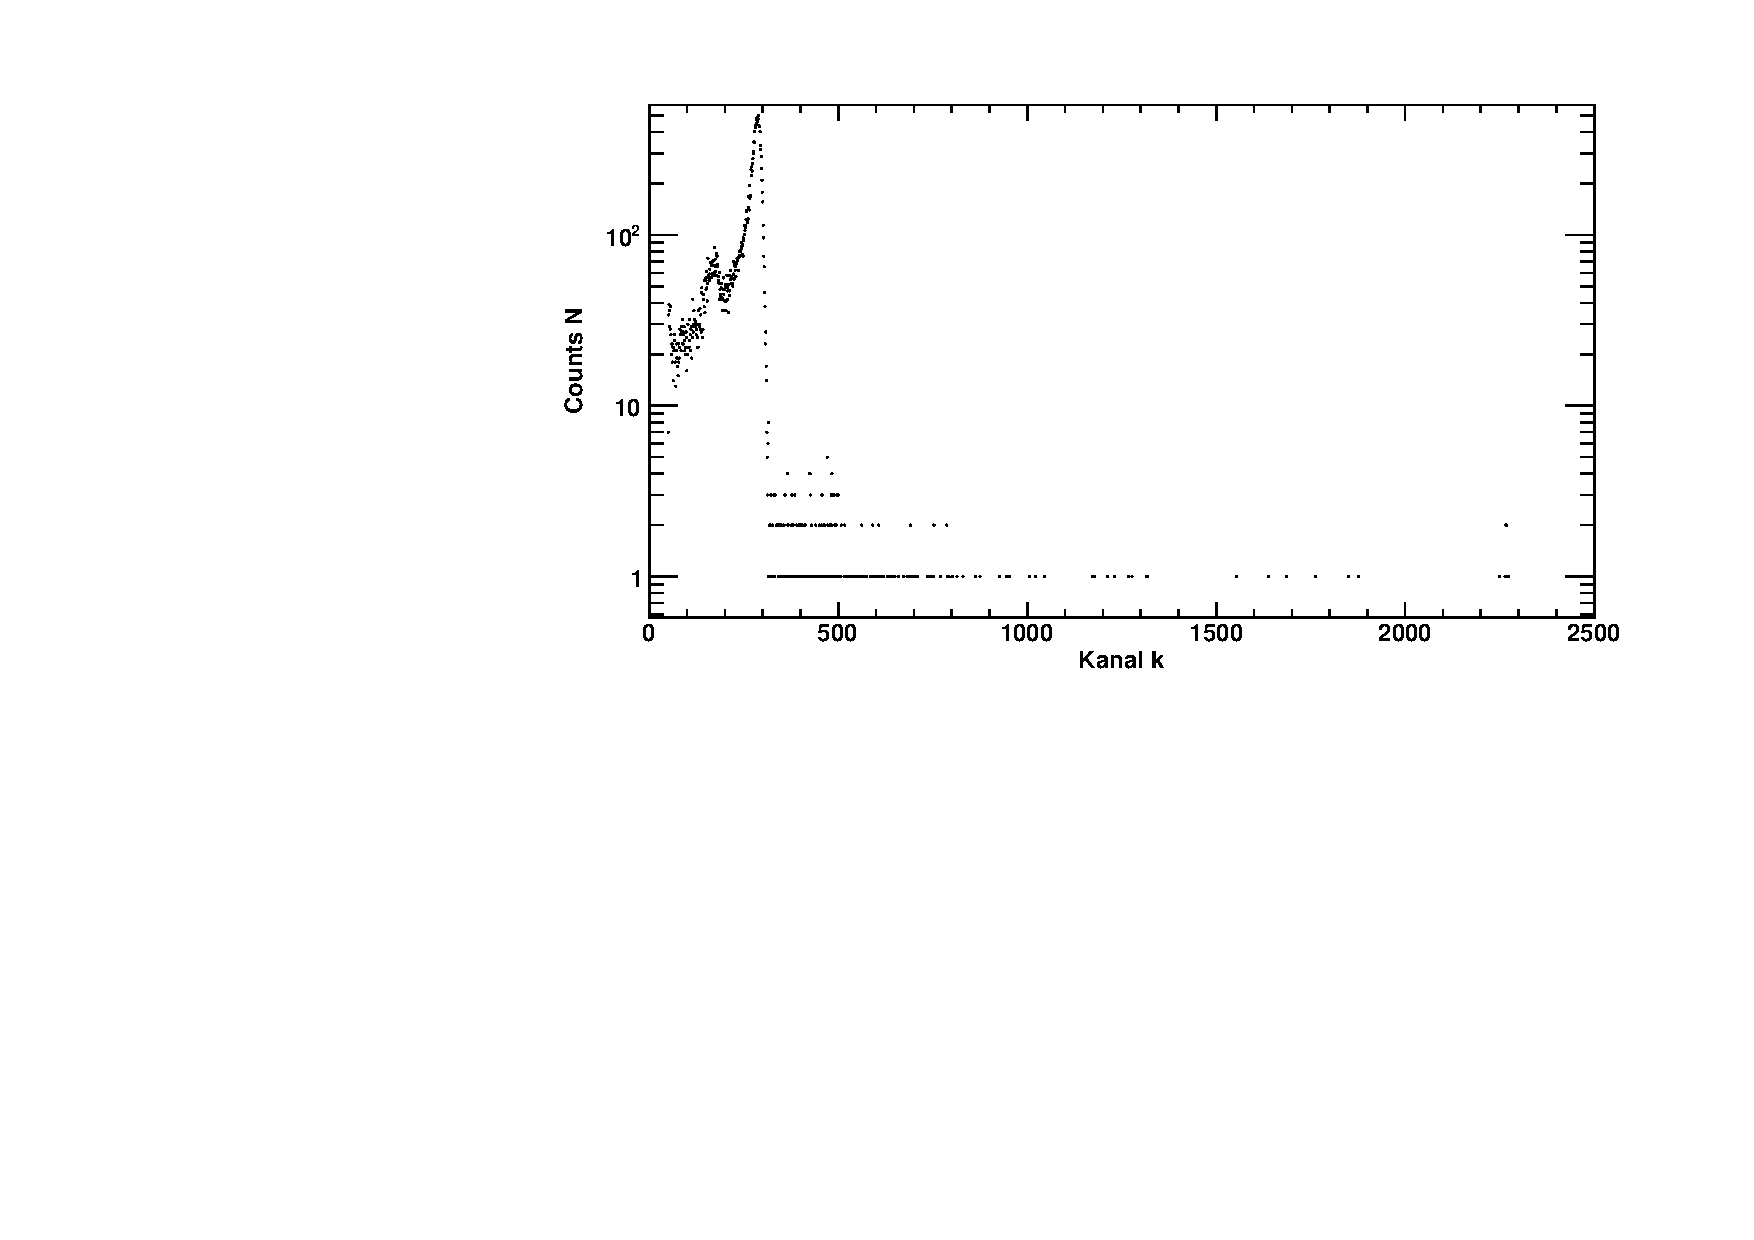
\includegraphics[width=0.95\textwidth]{../img/part3/Am-CdTe_spectrum.pdf}
  \caption{Spektrum von \am, gemessen mit dem CdTe-Detektor.}
  \label{img:cdte:am:spektrum}
\end{center}
\end{figure}


\paragraph{Peaks}
Die einzelnen Peaks werden mit einer normierten Gauß-Kurve gefittet.
\begin{equation}
  \label{eq:part3:normgauss}
  N(k) = A \cdot \frac{1}{\sqrt{2\pi \cdot \sigma^2}} \cdot e^{-\frac{1}{2} \left( \frac{k-k_c}{\sigma} \right)^2}
\end{equation}
Die Fits sind in \autoref{img:am:cdte:peak0}, \autoref{img:co:cdte:peak0} und \autoref{img:co:cdte:peak1} dargestellt. Wie man erkennt, sind die 
Peaks nicht ganz symmetrisch.
Durch die unterschiedliche Absorptionstiefe ist der Abstand zu Kathode und Anode nicht konstant, die 
entstandenen Ladungsträger rekombinieren teilweise wieder. Dieser Effekt soll jedoch nach \cite{staatsex} nicht berücksichtigt werden, die 
Peaks können in guter Näherung mit einer Gauß-Kurve gefittet werden.
\begin{figure}[H]
\begin{center}
  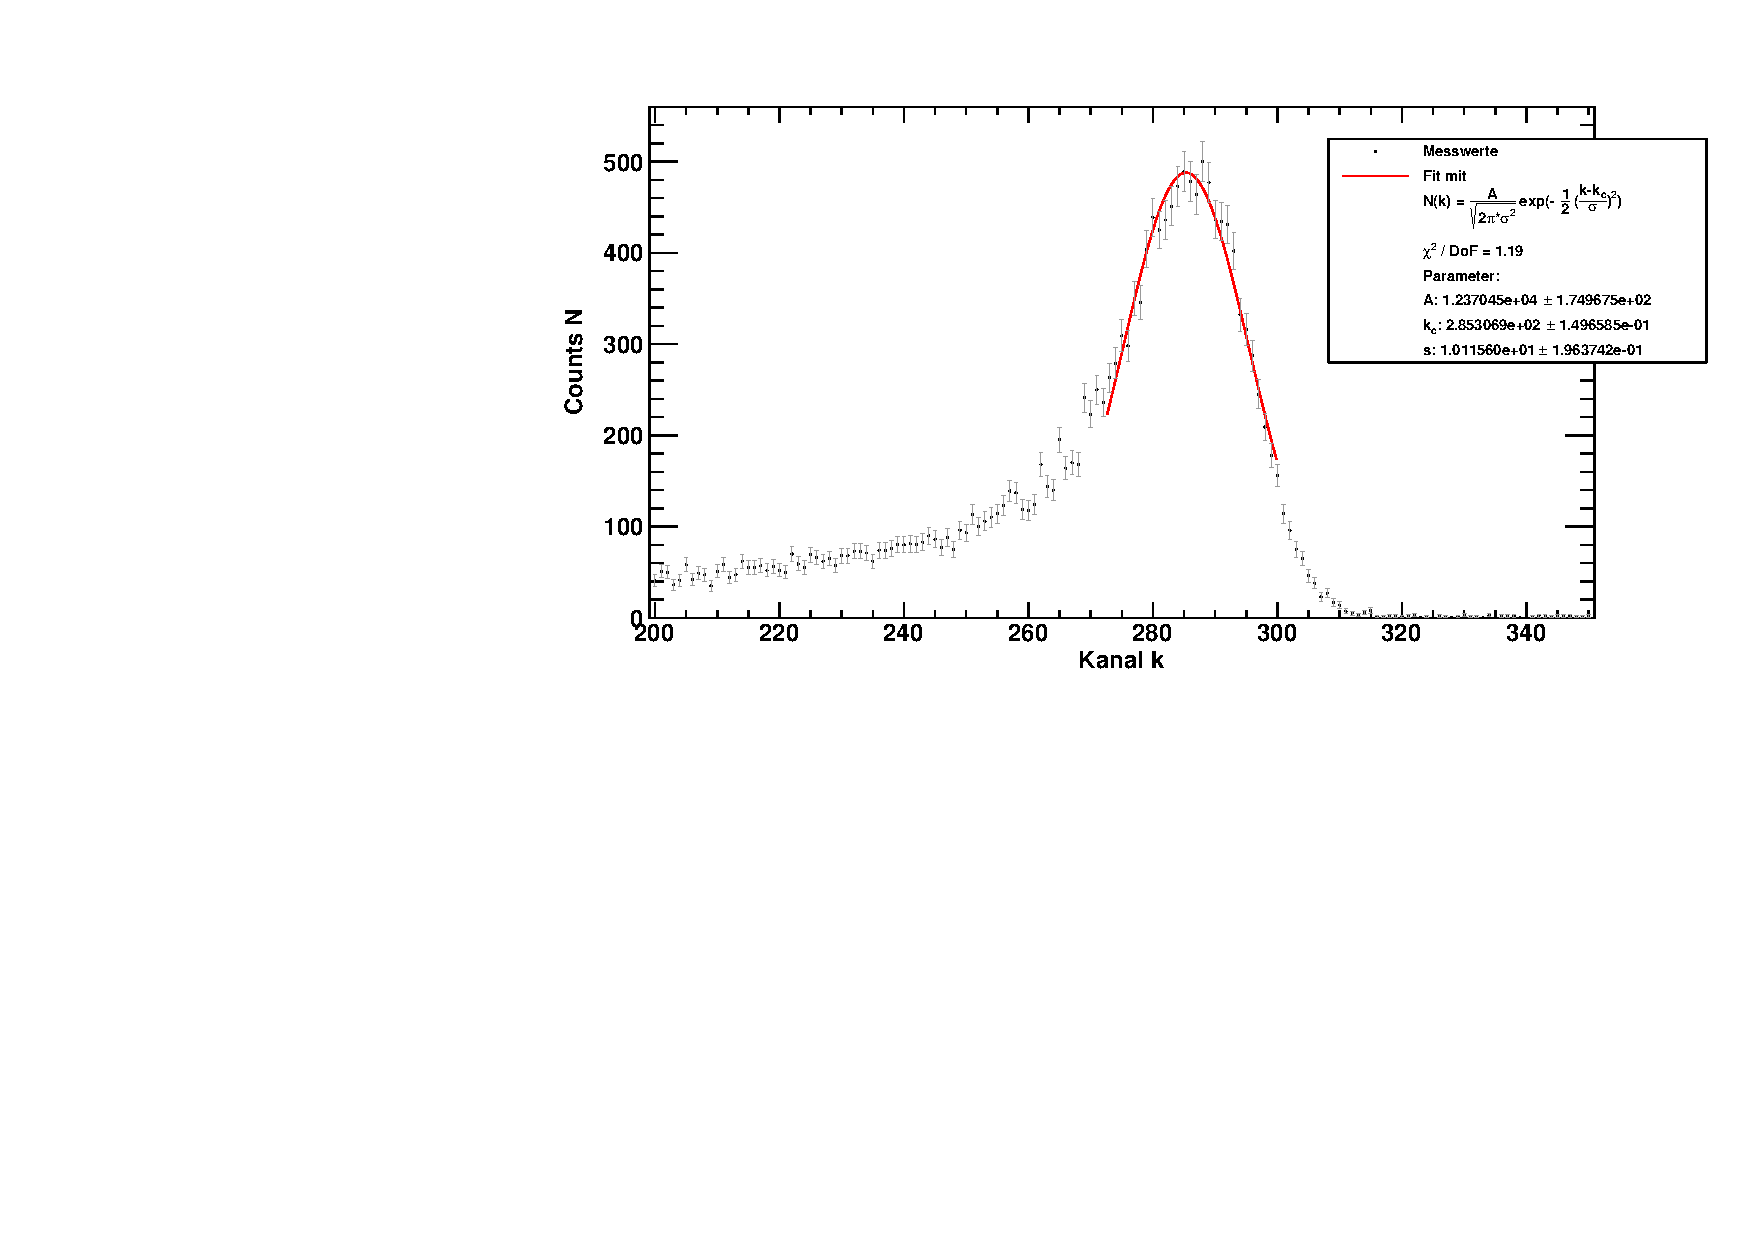
\includegraphics[width=\textwidth]{../img/part3/Am-CdTe_00.pdf}
  \caption{59.5\,keV-Peak von \am, gemessen mit dem CdTe-Detektor.}
  \label{img:am:cdte:peak0}
\end{center}
\end{figure}

\begin{figure}[H]
\begin{center}
  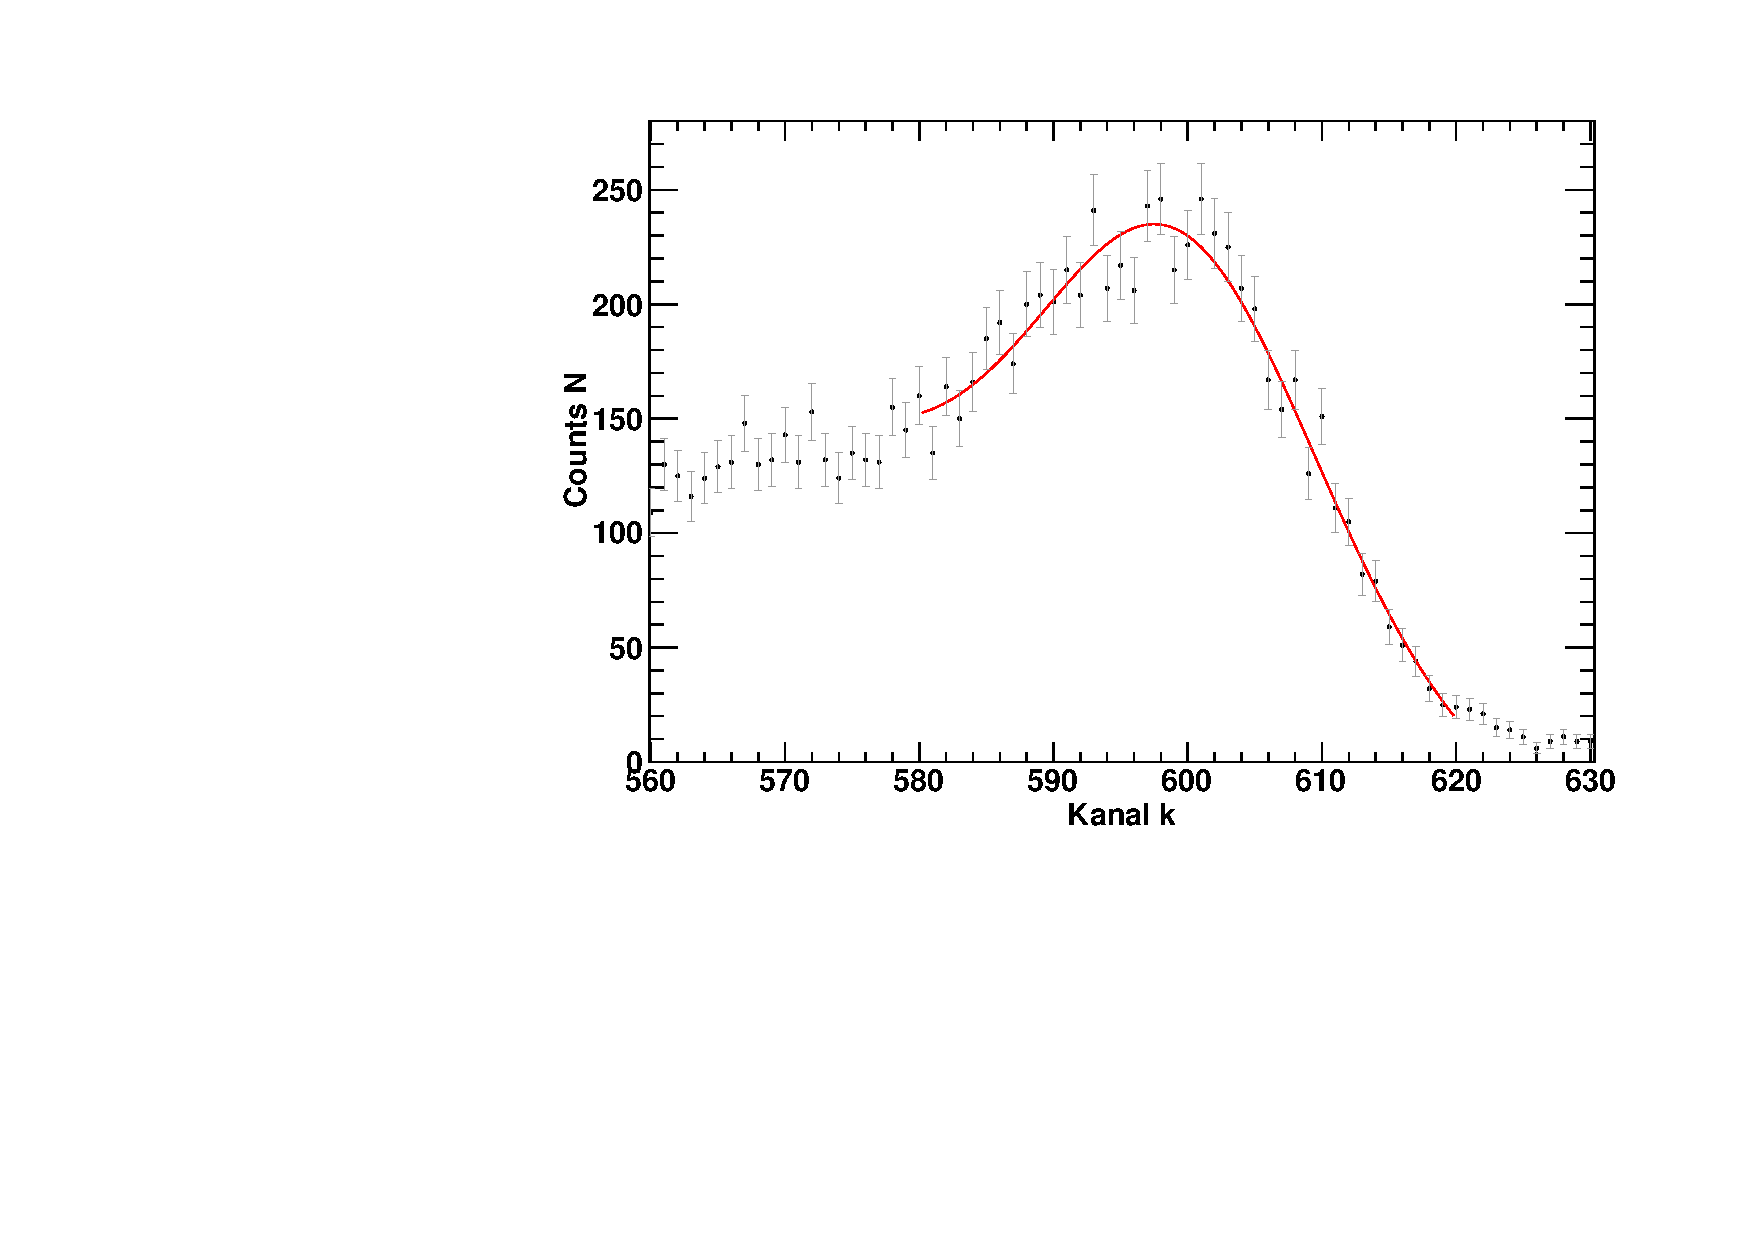
\includegraphics[width=\textwidth]{../img/part3/Co-CdTe_00.pdf}
  \caption{122.06\,keV-Peak von \co, gemessen mit dem CdTe-Detektor.}
  \label{img:co:cdte:peak0}
\end{center}
\end{figure}

\begin{figure}[H]
\begin{center}
  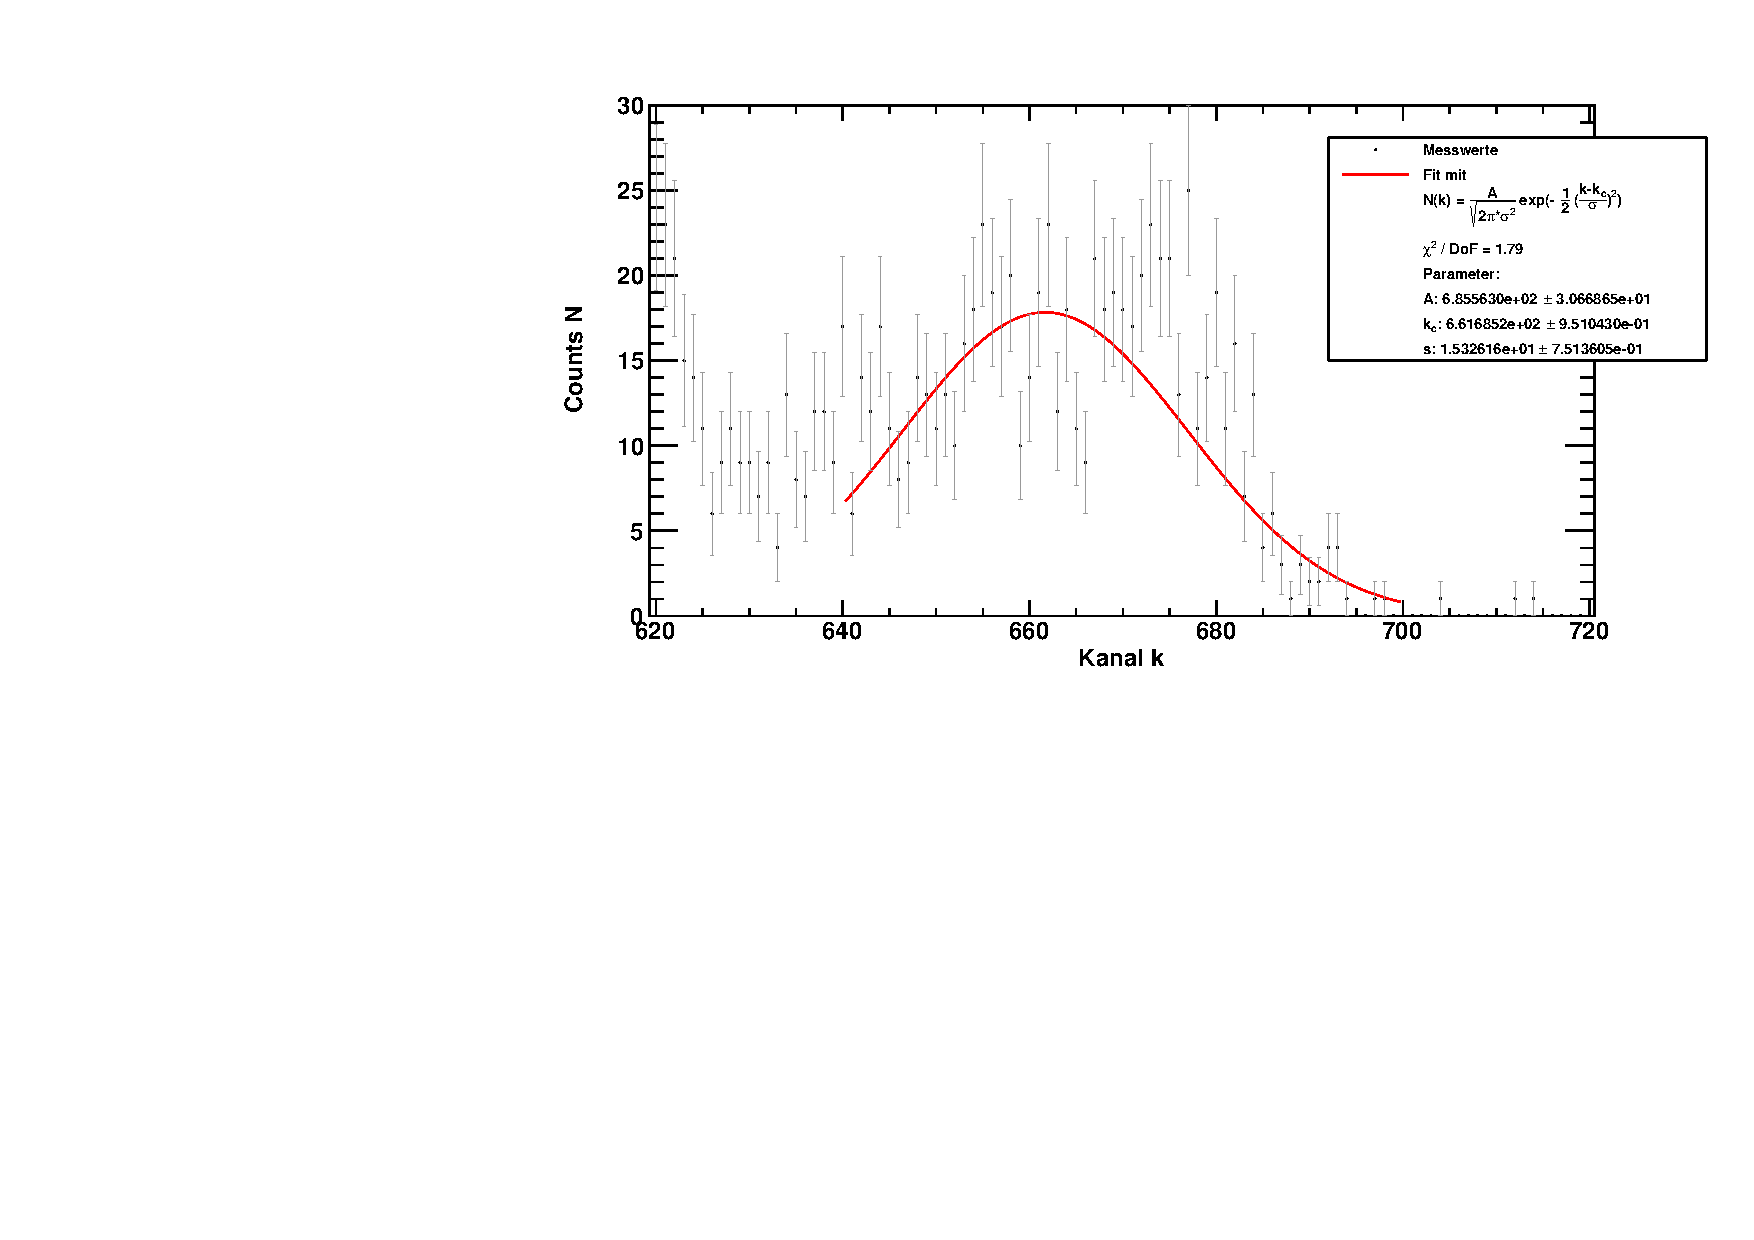
\includegraphics[width=\textwidth]{../img/part3/Co-CdTe_01.pdf}
  \caption{136.47\,keV-Peak von \co, gemessen mit dem CdTe-Detektor.}
  \label{img:co:cdte:peak1}
\end{center}
\end{figure}

\paragraph{Energieeichung}
Die Literaturwerte der Peaks werden über den oben erhaltenen Erwartungswerten der Gauß-Kurven aufgetragen. Dieser Graph ist Grundlage der 
Energieeichung (\autoref{img:cdte:energygauge}). Es wird eine lineare Abhängigkeit der gemessenen Energie $E$ von der Kanalnummer $k$ angenommen.
\begin{equation}
  E(k) = a + b \cdot k
\end{equation}
Man erhält für die Parameter:
\begin{equation}
\begin{split}
  a &= (1.86 \pm 0.09)\,\text{eV} \\
  b &= (0.2020 \pm 0.0003)\,\text{eV}
\end{split}
\end{equation}
\begin{figure}[H]
\begin{center}
  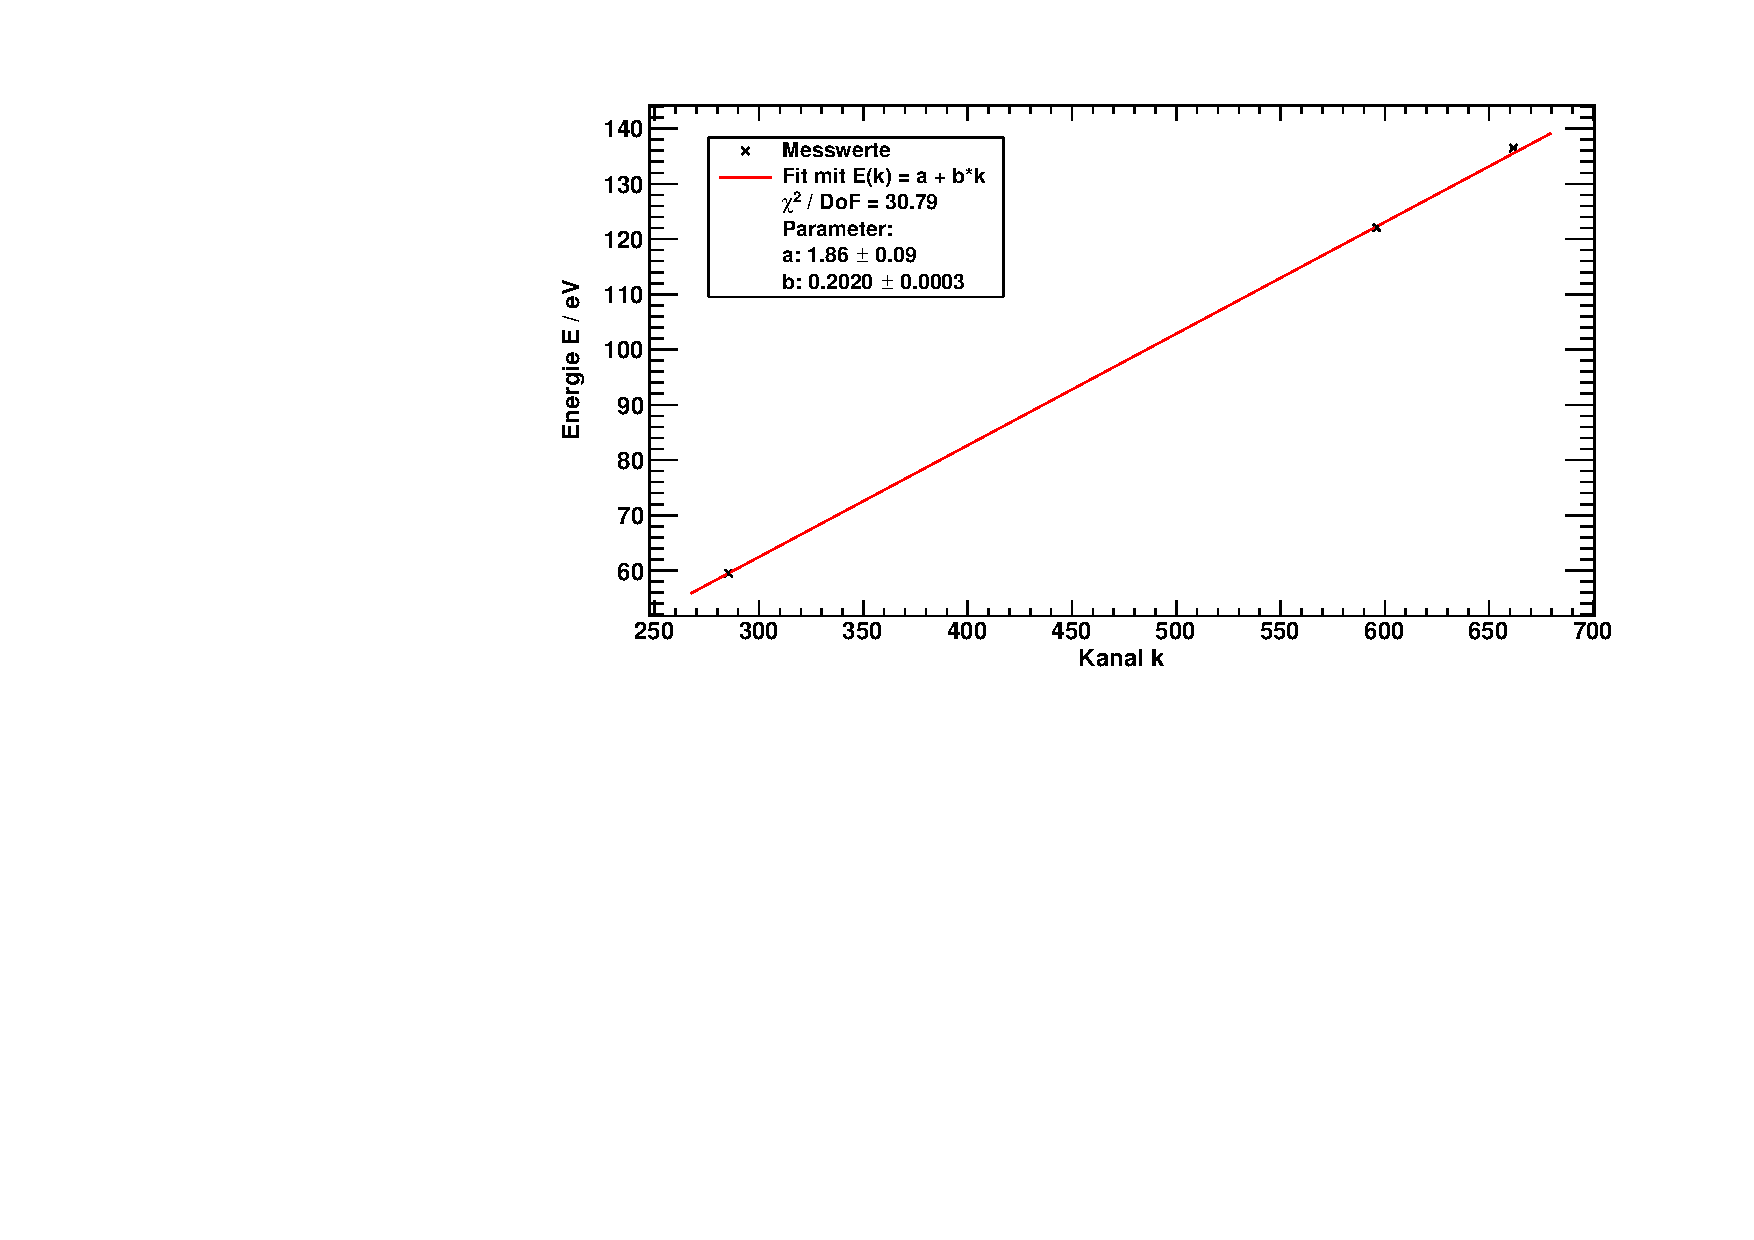
\includegraphics[width=\textwidth]{../img/part3/energygauge_CdTe.pdf}
  \caption{Energieeichung des CdTe-Detektors.}
  \label{img:cdte:energygauge}
\end{center}
\end{figure}
Der hohe Wert des $\chi^2$ kann mit einer Nichtlinearität des Detektors oder des MCA erklärt werden. Allerdings ist ein quadratischer Fit 
(vermutetes Modell) bei nur drei Messpunkten nicht sinnvoll, da die Anzahl der einzelnen Messpunkte der Anzahl der Fitparameter entspricht, es 
gibt dann keinen Freiheitsgrad.
Die Fehler der Messpunkte stammen aus den Fits (die akzeptable $\chi^2$-Werte besitzen). Die Counts 
wurden wie oben beschrieben als poissonverteilt angenommen.

\paragraph{Relative Energieauflösung}
Die relativen Energieauflösungen wurden aus der Position $k_c$ und der Standardabweichung bestimmt (\autoref{tab:cdte:rer}). 
\begin{equation}
  \label{eq:rer}
  \text{RER} = \frac{2 \sqrt{2 \ln(2)} \cdot \sigma}{k_c} 
\end{equation}
\begin{table}[H]
\begin{center}
\begin{tabular}{|c|c|}
\hline 
Kanal & RER \\ \hline
285.31 $\pm$ 0.15 & 0.0835 $\pm$ 0.0016\\ \hline
596.1 $\pm$ 0.4 & 0.055 $\pm$ 0.003 \\ \hline
661.7 $\pm$ 1.0 & 0.055 $\pm$ 0.003 \\ \hline
\end{tabular}
\caption{Energieauflösungen des CdTe-Detektors}
\label{tab:cdte:rer}
\end{center}
\end{table}

\subsubsection{Si-Detektor}
\paragraph{Spektren}
In den Spektren von \co\ und \am\ (\autoref{img:si:co:spektrum} und \autoref{img:si:am:spektrum}) sieht den 59.5\,keV-Peak 
von \am\, bei Kanal 300 und den 122.06\,keV-Peak von \co\, bei Kanal 600. Der 136.47\,keV-Peak von \co\, lässt sich im Gesamtspektrum 
ohne Vergrößerung (der x-Achse) nicht mehr erkennen, er lässt sich allerdings direkt rechts neben dem 122.06\,keV-Peak finden.
\begin{figure}[H]
\begin{center}
  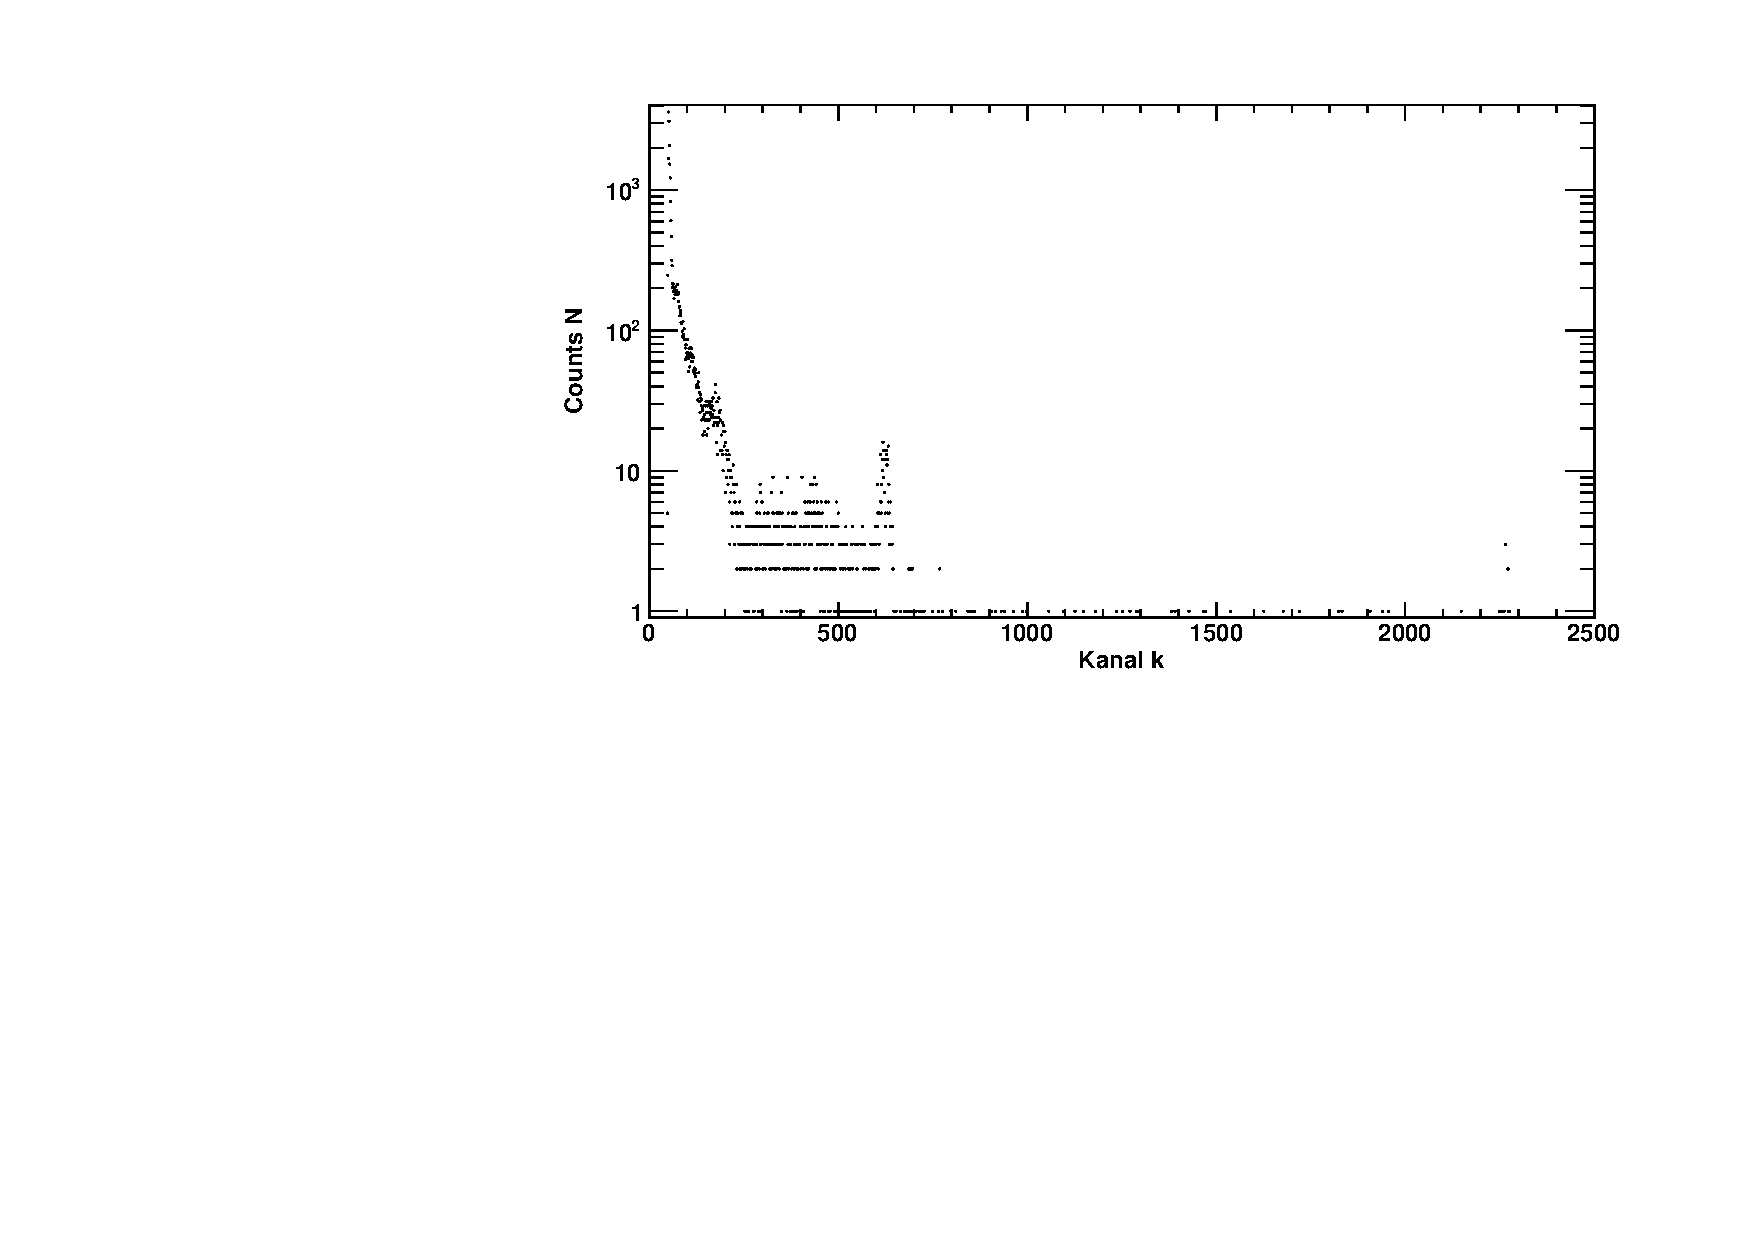
\includegraphics[width=\textwidth]{../img/part3/Co-Si_spectrum.pdf}
  \caption{Spektrum von \co, gemessen mit dem Si-Detektor.}
  \label{img:si:co:spektrum}
\end{center}
\end{figure}

\begin{figure}[H]
\begin{center}
  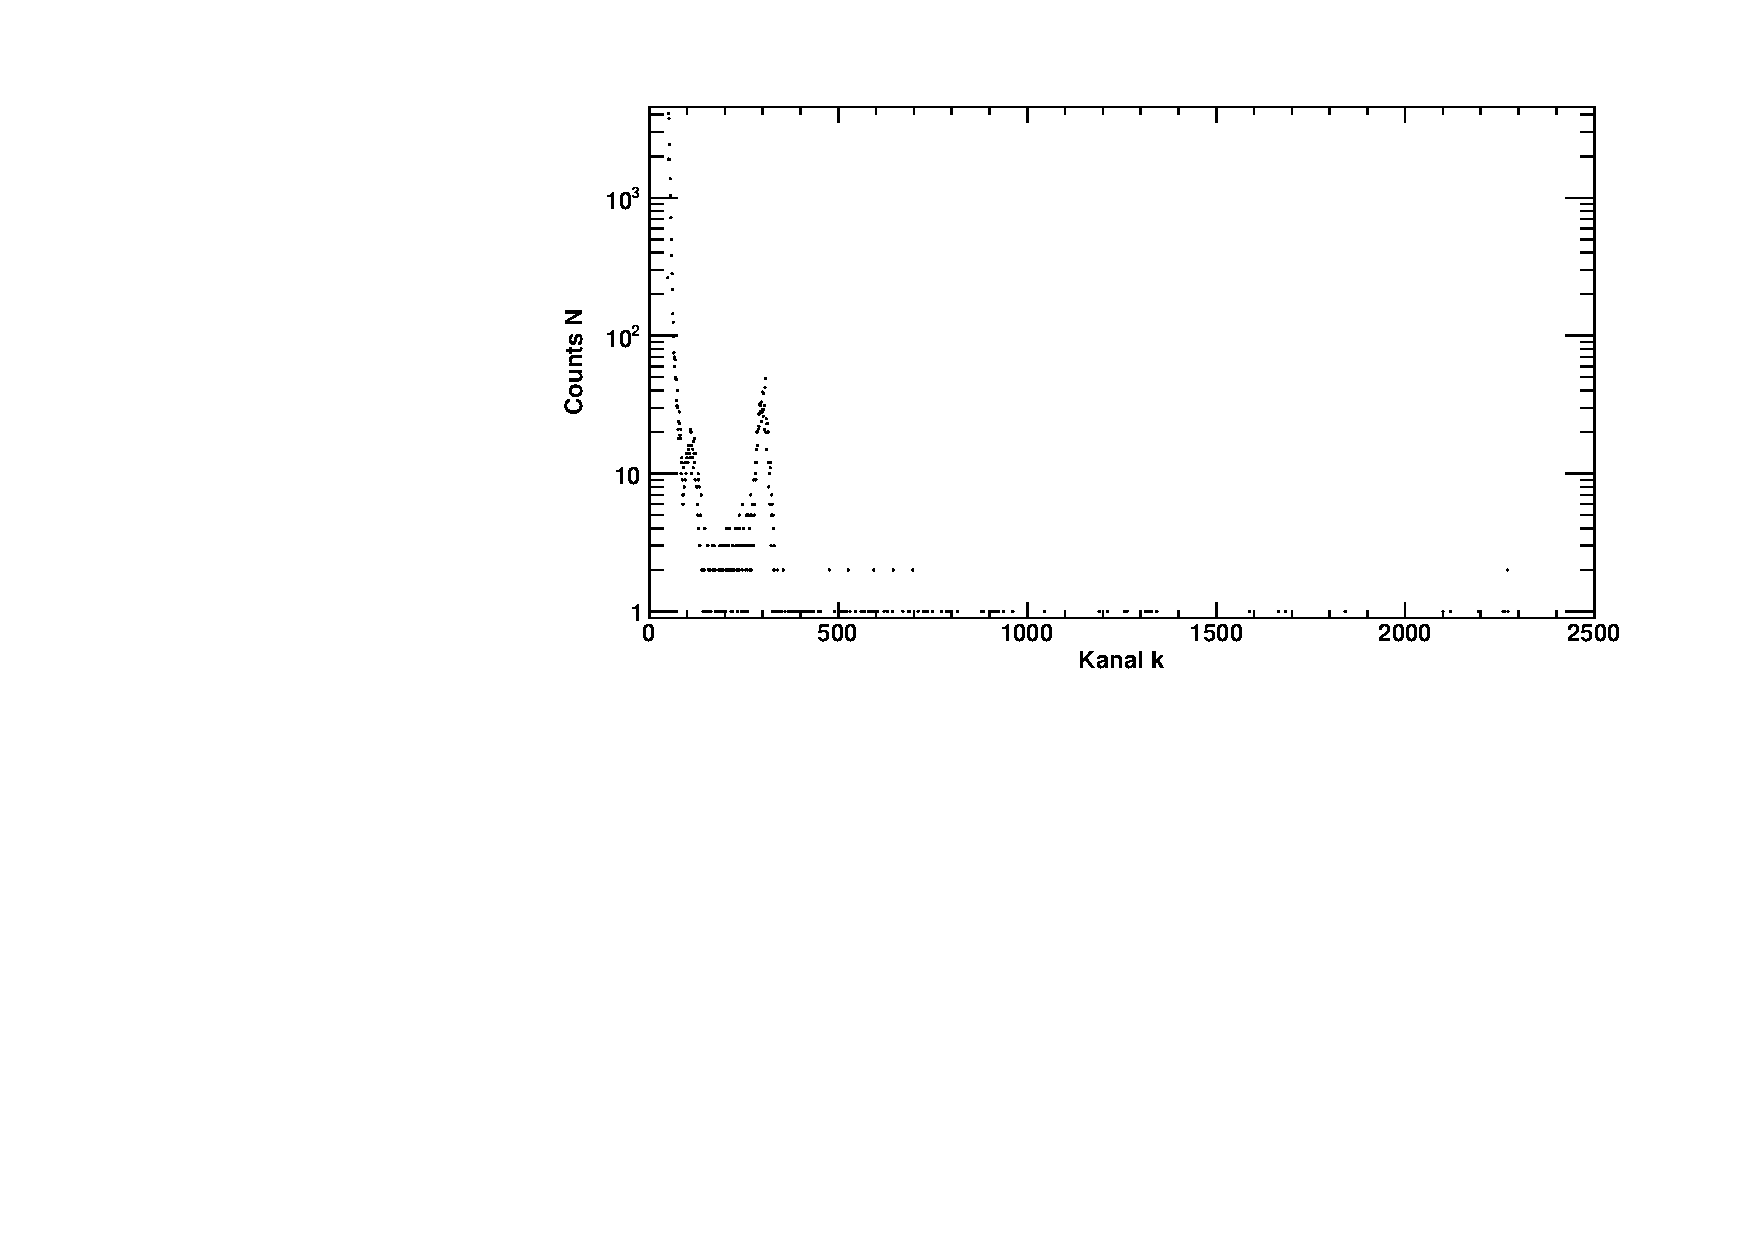
\includegraphics[width=\textwidth]{../img/part3/Am-Si_spectrum.pdf}
  \caption{Spektrum von \am, gemessen mit dem Si-Detektor.}
  \label{img:si:am:spektrum}
\end{center}
\end{figure}

\paragraph{Peaks}
Die Peaks werden wieder mit der normierten Gaußkurve (\autoref{eq:part3:normgauss}) gefittet 
(\autoref{img:am:si:peak0}, \autoref{img:co:si:peak0} und \autoref{img:co:si:peak1}). Jedoch hat der 136.47\,keV-Peak von \co\ eine zu kleine 
Anzahl von Counts, dass man noch gut eine Gaußkurve erkennen und anpassen kann. Im nächsten Abschnitt wird erklärt, wie man doch noch 
Informationen über die Lage und Ausdehnung des Peaks erhalten kann.
\begin{figure}[H]
\begin{center}
  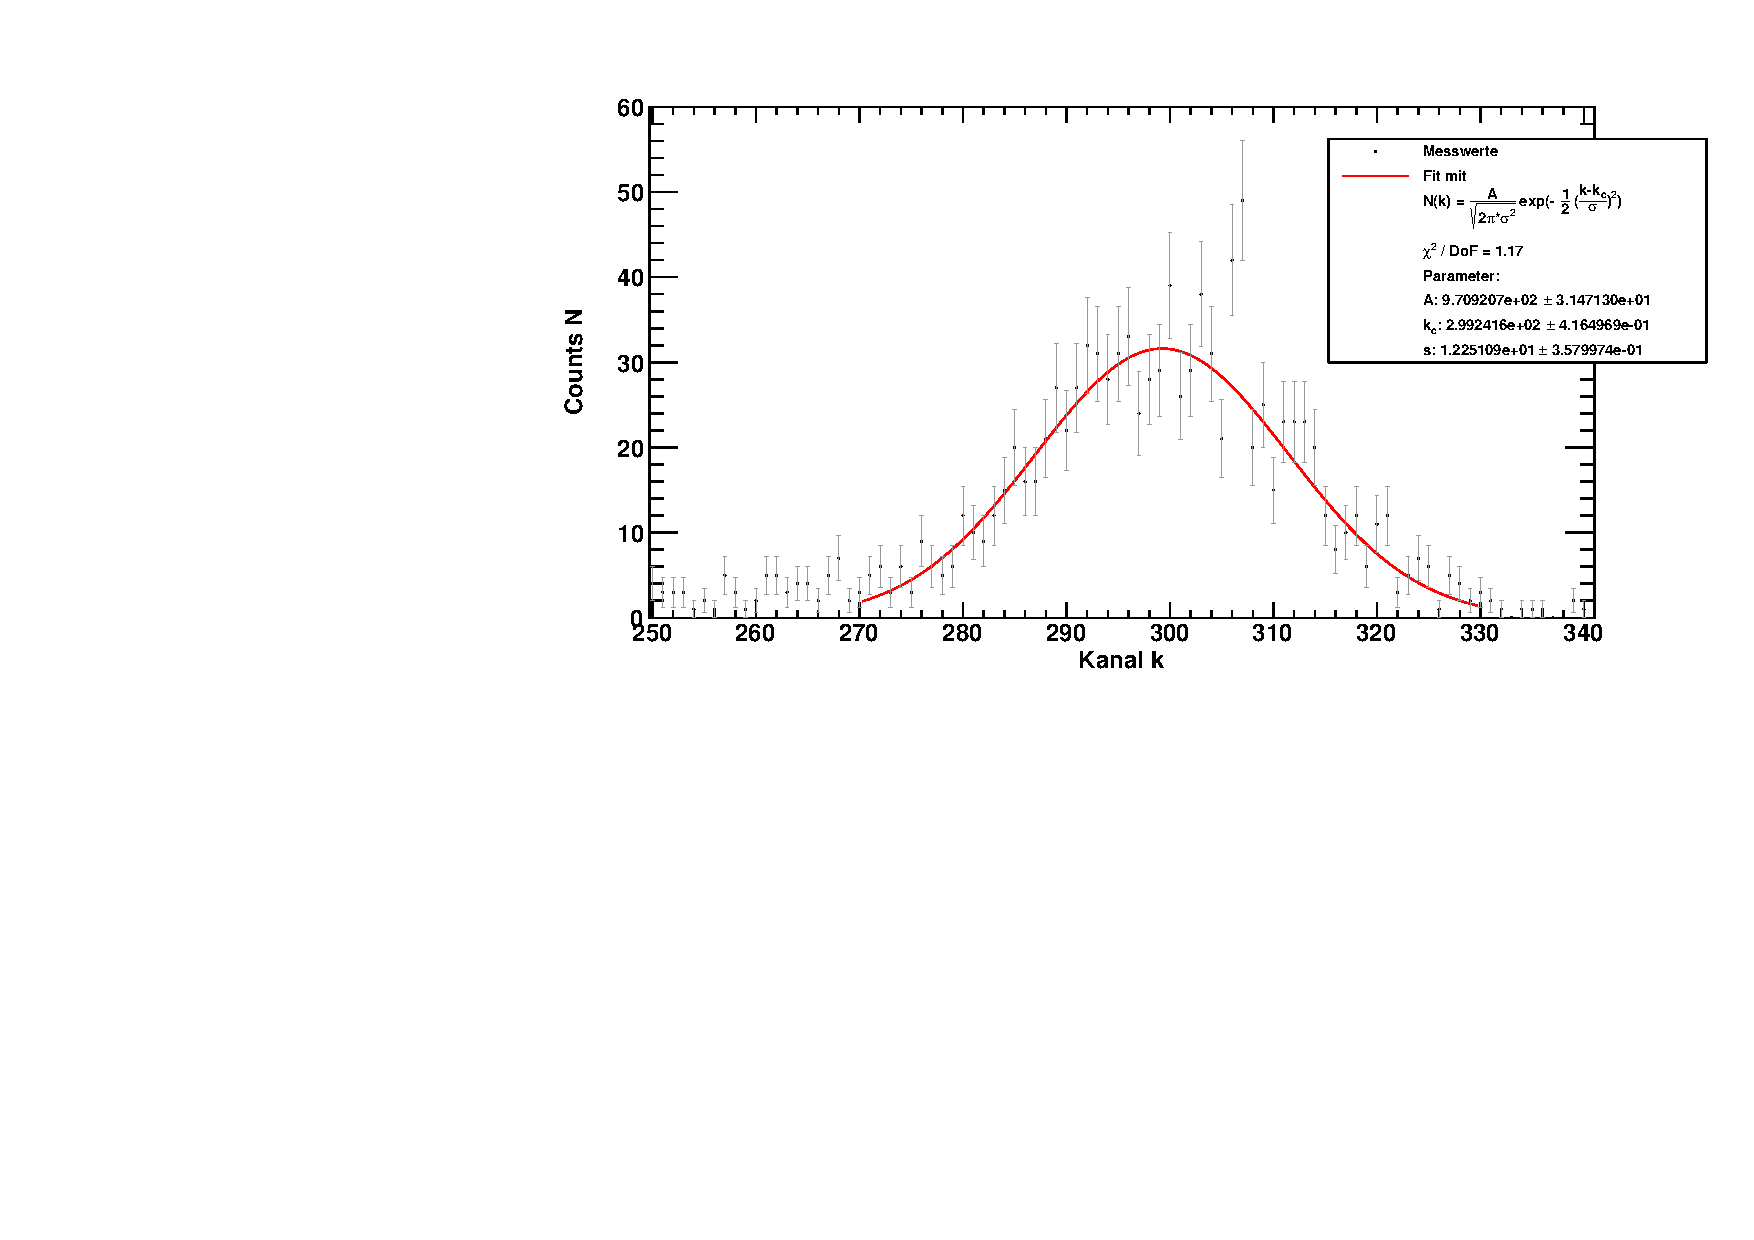
\includegraphics[width=\textwidth]{../img/part3/Am-Si_00.pdf}
  \caption{59.5\,keV-Peak von \am, gemessen mit dem Si-Detektor.}
  \label{img:am:si:peak0}
\end{center}
\end{figure}

\begin{figure}[H]
\begin{center}
  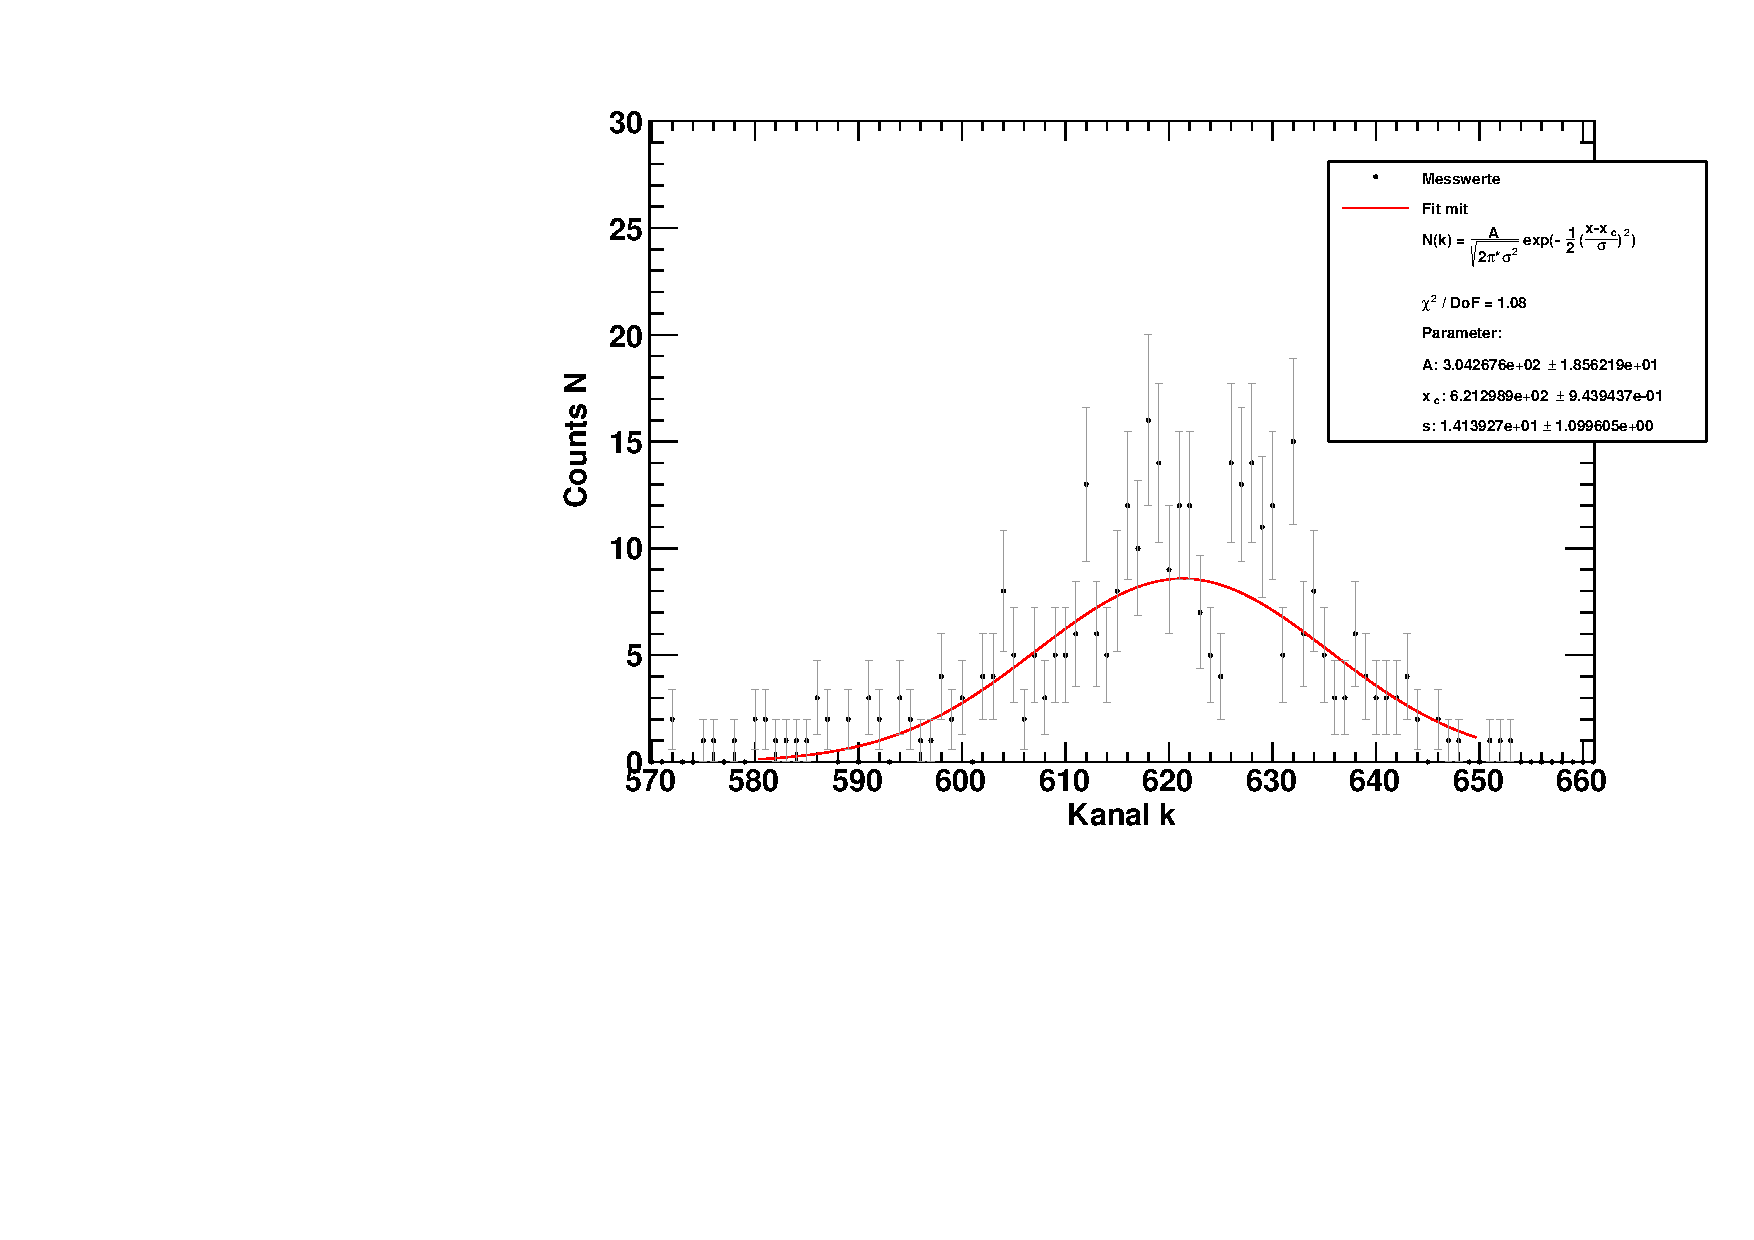
\includegraphics[width=\textwidth]{../img/part3/Co-Si_00.pdf}
  \caption{122.06\,keV-Peak von \co, gemessen mit dem Si-Detektor.}
  \label{img:co:si:peak0}
\end{center}
\end{figure}

\begin{figure}[H]
\begin{center}
  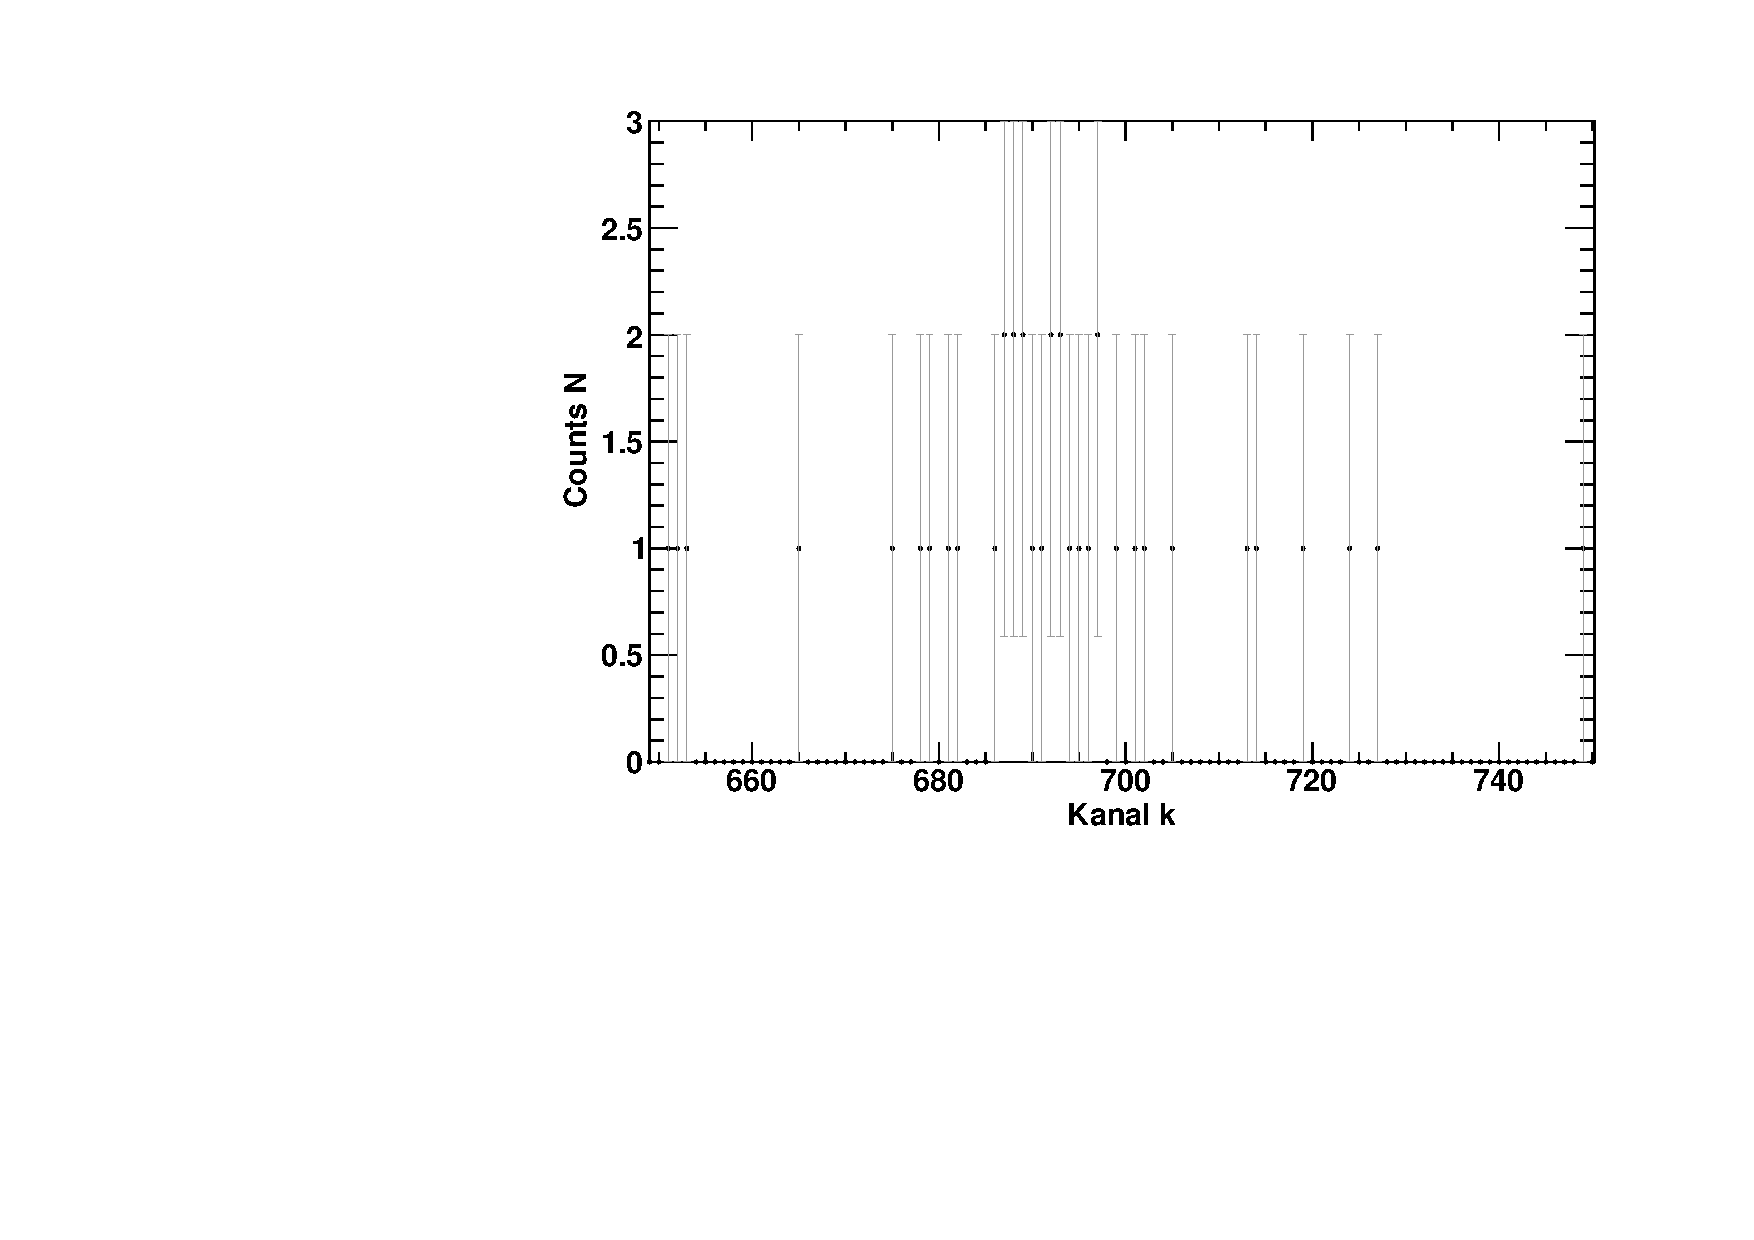
\includegraphics[width=\textwidth]{../img/part3/Co-Si_01.pdf}
  \caption{136.47\,keV-Peak von \co, gemessen mit dem Si-Detektor.}
  \label{img:co:si:peak1}
\end{center}
\end{figure}

\paragraph{Bestimmung des 136.47\,keV-Peak von \co}
Um doch noch den 136.47\,keV-Peak von \co\ fitten zu können wird jeweils von 5 Kanälen der Mittelwert der Kanäle und der Counts gebildet. 
Die Fehler werden mit Gauß'scher Fehlerfortpflanzung berechnet.
Das so erhaltene Spektrum zeigt einen klar erkennbaren Peak, der sich auch fitten lässt (\autoref{img:co:si:peak1:merged}).
\begin{figure}[H]
\begin{center}
  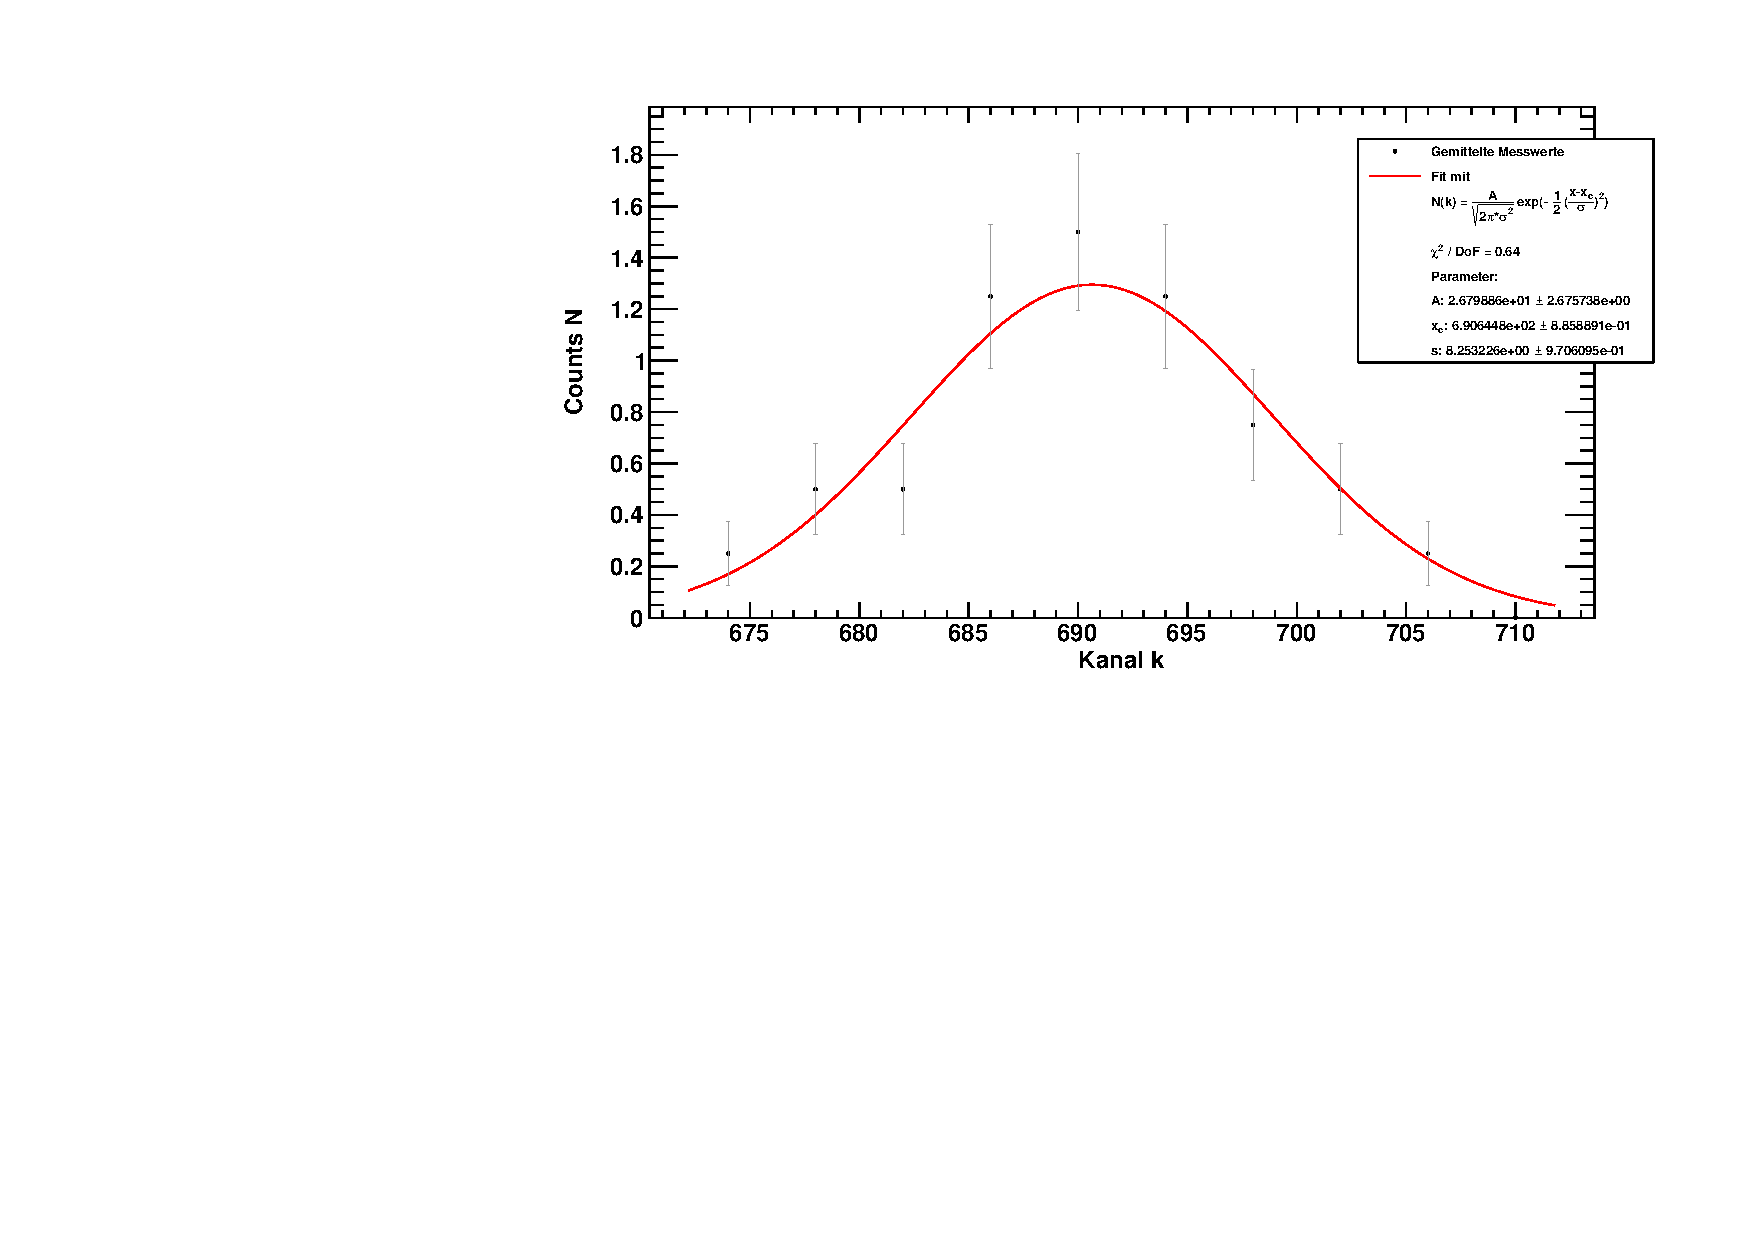
\includegraphics[width=\textwidth]{../img/part3/Co-Si_01_mergedbins.pdf}
  \caption{136.47\,keV-Peak von \co, gemessen mit dem Si-Detektor. Jeweils 5 Kanäle wurden zusammengefasst.}
  \label{img:co:si:peak1:merged}
\end{center}
\end{figure}

\paragraph{Energieeichung}
Die Energieeichung des Si-Detektors erfolgt analog zu derjenigen des CdTe-Detektors.
\begin{equation}
    E(k) = a + b\cdot k
\end{equation}
\begin{figure}[H]
\begin{center}
  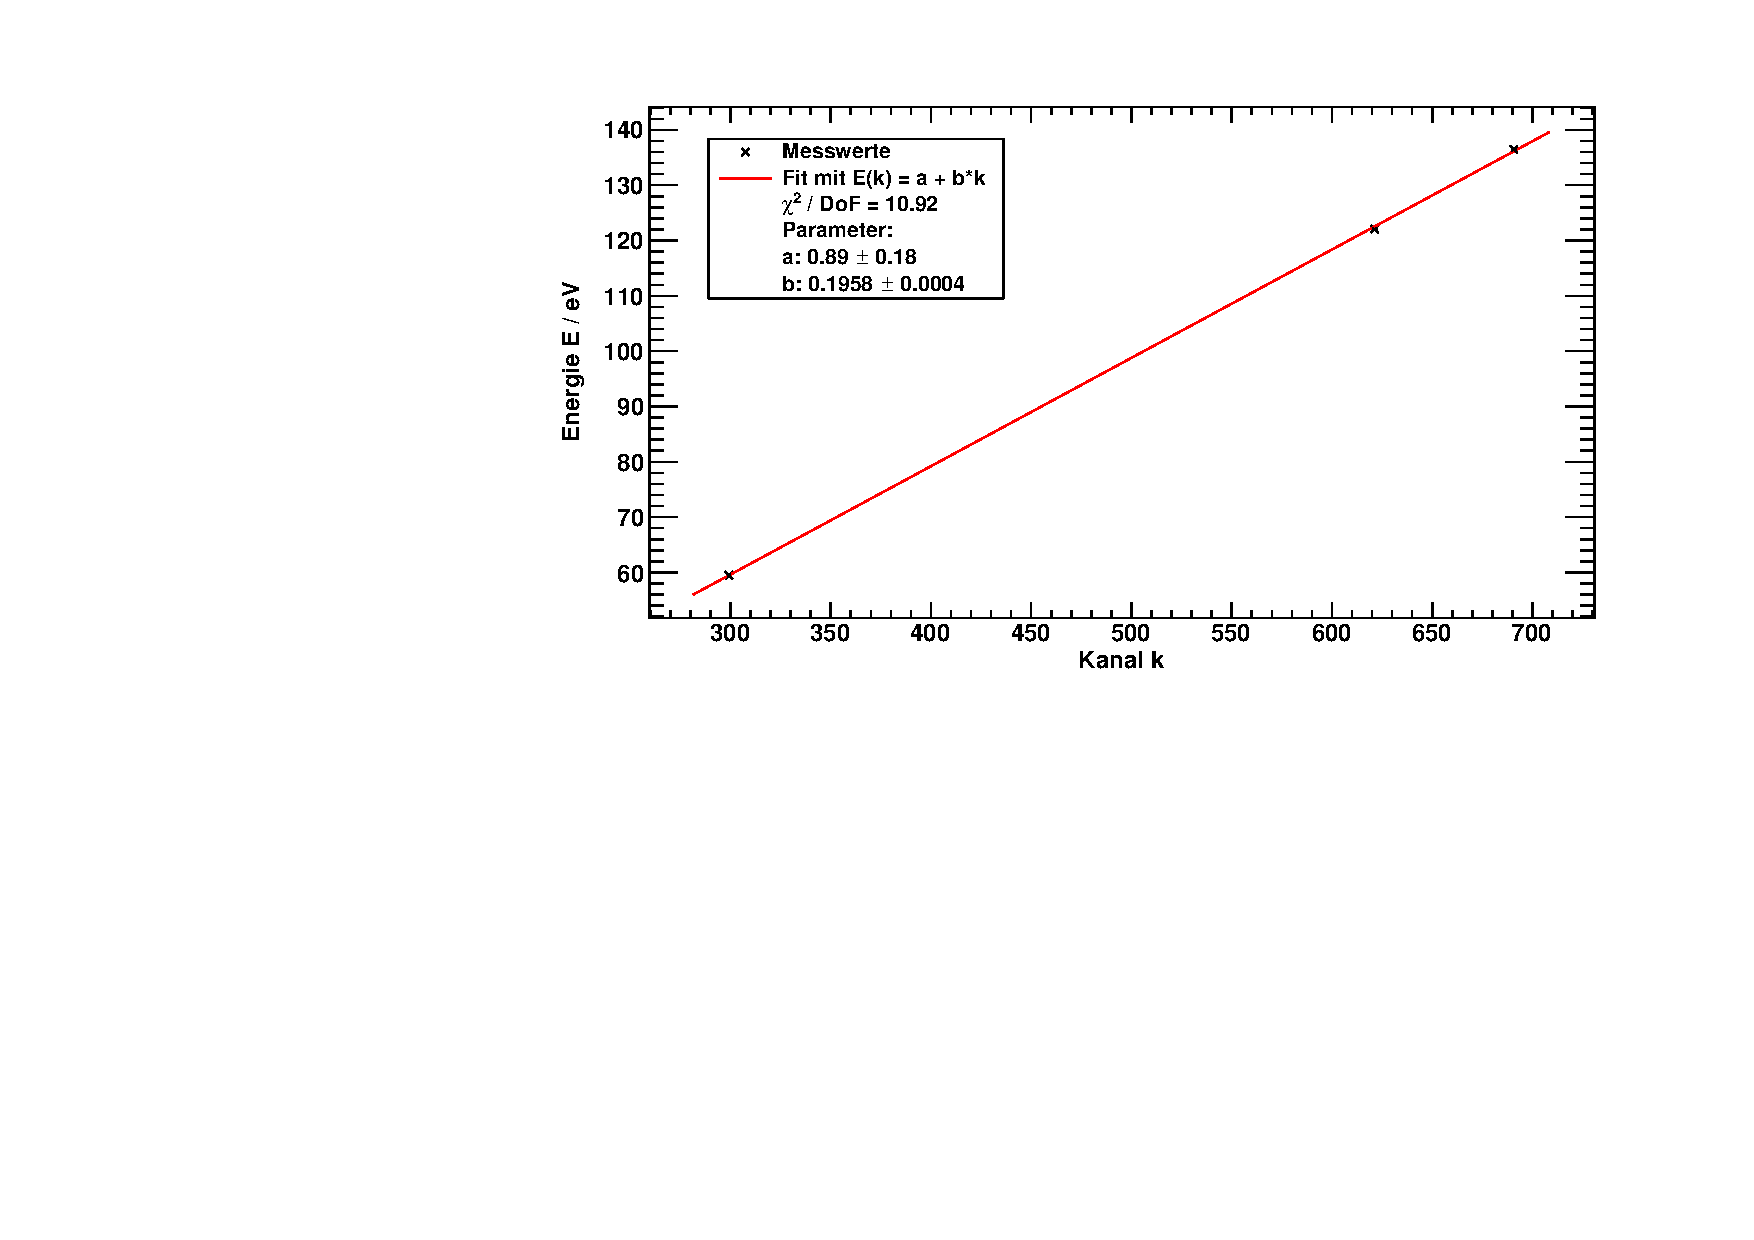
\includegraphics[width=\textwidth]{../img/part3/energygauge_Si.pdf}
  \caption{Energieeichung des Si-Detektors.}
  \label{img:si:energygauge}
\end{center}
\end{figure}
Es folgt für die Paramter:
\begin{equation}
\begin{split}
  a &= (0.89 \pm 0.18)\,\text{eV} \\
  b &= (0.1958 \pm 0.0004)\,\text{eV}
\end{split}
\end{equation}
Sie haben einen ähnlichen Wert wie die des CdTe-Detektors. 
Das $\chi^2$ ist hier ebenfalls aus den oben beschriebenen Gründen erhöht.

\paragraph{Relative Energieauflösung}
Die relative Energieauflösung des Si-Detektors wird mit \autoref{eq:rer} für jeden Peak bestimmt (\autoref{tab:si:rer}), 
die Parameter folgen aus den Fits.
\begin{table}[H]
\begin{center}
\begin{tabular}{|c|c|}
\hline 
Kanal & RER \\ \hline
299.2 $\pm$ 0.4 & 0.096 $\pm$ 0.003 \\ \hline
621.3 $\pm$ 0.9 & 0.054 $\pm$ 0.004 \\ \hline
690.6 $\pm$ 0.9 & 0.028 $\pm$ 0.003 \\ \hline
\end{tabular}
\caption{Energieauflösungen des Si-Detektors.}
\label{tab:si:rer}
\end{center}
\end{table}

\subsubsection{Absorptionsverhältnisse}
Die Absorptionswahrscheinlichkeit lässt sich mit der Amplitude $A$ aus dem Gauß-Fit und der Detektoroberfläche $a$ bestimmen: 
\begin{equation}
  \text{Abs} = \frac{A}{a}
\end{equation}
Der Quotient aus der Absorptionswahrscheinlichkeit der beiden Detektoren bei gleicher Energie liefert das Absorptionsverhältnis 
(\autoref{tab:absrel}).
\begin{table}[H]
\begin{center}
\begin{tabular}{|c|c|c|}
\hline 
Energie & $\text{Abs}_{\text{Si}} / \text{Abs}_{\text{CdTe}}$ & Literaturwert \cite{staatsex} \\ \hline
59.5 & 0.0181    $\pm$ 0.0006 & 0.0140 \\ \hline
122.06 & 0.0087 $\pm$ 0.0007 & 0.0183 \\ \hline
136.47 & 0.0090 $\pm$ 0.0010 & 0.0200 \\ \hline
\end{tabular}
\caption{Absorptionsverhältnisse von Si- und CdTe-Detektor.}
\label{tab:absrel}
\end{center}
\end{table}
Die berechneten Werte stimmen nicht mit den Literaturwerten \cite{staatsex} überein. Dies kann mehrerer Gründe haben 
(beschrieben in \cite{staatsex}), wie zum Beispiel Absorption der Epoxid- und $\text{SiO}_2$-Schicht oder Ladungsrekombination. Jedoch 
stimmt die Vorrausage von \cite{staatsex}, dass die gemessenen Werte etwa um den Faktor 2 von den Literaturwerten abweichen, für die beiden Peaks 
mit höherer Energie.